\documentclass[1p]{elsarticle_modified}
%\bibliographystyle{elsarticle-num}

%\usepackage[colorlinks]{hyperref}
%\usepackage{abbrmath_seonhwa} %\Abb, \Ascr, \Acal ,\Abf, \Afrak
\usepackage{amsfonts}
\usepackage{amssymb}
\usepackage{amsmath}
\usepackage{amsthm}
\usepackage{scalefnt}
\usepackage{amsbsy}
\usepackage{kotex}
\usepackage{caption}
\usepackage{subfig}
\usepackage{color}
\usepackage{graphicx}
\usepackage{xcolor} %% white, black, red, green, blue, cyan, magenta, yellow
\usepackage{float}
\usepackage{setspace}
\usepackage{hyperref}

\usepackage{tikz}
\usetikzlibrary{arrows}

\usepackage{multirow}
\usepackage{array} % fixed length table
\usepackage{hhline}

%%%%%%%%%%%%%%%%%%%%%
\makeatletter
\renewcommand*\env@matrix[1][\arraystretch]{%
	\edef\arraystretch{#1}%
	\hskip -\arraycolsep
	\let\@ifnextchar\new@ifnextchar
	\array{*\c@MaxMatrixCols c}}
\makeatother %https://tex.stackexchange.com/questions/14071/how-can-i-increase-the-line-spacing-in-a-matrix
%%%%%%%%%%%%%%%

\usepackage[normalem]{ulem}

\newcommand{\msout}[1]{\ifmmode\text{\sout{\ensuremath{#1}}}\else\sout{#1}\fi}
%SOURCE: \msout is \stkout macro in https://tex.stackexchange.com/questions/20609/strikeout-in-math-mode

\newcommand{\cancel}[1]{
	\ifmmode
	{\color{red}\msout{#1}}
	\else
	{\color{red}\sout{#1}}
	\fi
}

\newcommand{\add}[1]{
	{\color{blue}\uwave{#1}}
}

\newcommand{\replace}[2]{
	\ifmmode
	{\color{red}\msout{#1}}{\color{blue}\uwave{#2}}
	\else
	{\color{red}\sout{#1}}{\color{blue}\uwave{#2}}
	\fi
}

\newcommand{\Sol}{\mathcal{S}} %segment
\newcommand{\D}{D} %diagram
\newcommand{\A}{\mathcal{A}} %arc


%%%%%%%%%%%%%%%%%%%%%%%%%%%%%5 test

\def\sl{\operatorname{\textup{SL}}(2,\Cbb)}
\def\psl{\operatorname{\textup{PSL}}(2,\Cbb)}
\def\quan{\mkern 1mu \triangleright \mkern 1mu}

\theoremstyle{definition}
\newtheorem{thm}{Theorem}[section]
\newtheorem{prop}[thm]{Proposition}
\newtheorem{lem}[thm]{Lemma}
\newtheorem{ques}[thm]{Question}
\newtheorem{cor}[thm]{Corollary}
\newtheorem{defn}[thm]{Definition}
\newtheorem{exam}[thm]{Example}
\newtheorem{rmk}[thm]{Remark}
\newtheorem{alg}[thm]{Algorithm}

\newcommand{\I}{\sqrt{-1}}
\begin{document}

%\begin{frontmatter}
%
%\title{Boundary parabolic representations of knots up to 8 crossings}
%
%%% Group authors per affiliation:
%\author{Yunhi Cho} 
%\address{Department of Mathematics, University of Seoul, Seoul, Korea}
%\ead{yhcho@uos.ac.kr}
%
%
%\author{Seonhwa Kim} %\fnref{s_kim}}
%\address{Center for Geometry and Physics, Institute for Basic Science, Pohang, 37673, Korea}
%\ead{ryeona17@ibs.re.kr}
%
%\author{Hyuk Kim}
%\address{Department of Mathematical Sciences, Seoul National University, Seoul 08826, Korea}
%\ead{hyukkim@snu.ac.kr}
%
%\author{Seokbeom Yoon}
%\address{Department of Mathematical Sciences, Seoul National University, Seoul, 08826,  Korea}
%\ead{sbyoon15@snu.ac.kr}
%
%\begin{abstract}
%We find all boundary parabolic representation of knots up to 8 crossings.
%
%\end{abstract}
%\begin{keyword}
%    \MSC[2010] 57M25 
%\end{keyword}
%
%\end{frontmatter}

%\linenumbers
%\tableofcontents
%
\newcommand\colored[1]{\textcolor{white}{\rule[-0.35ex]{0.8em}{1.4ex}}\kern-0.8em\color{red} #1}%
%\newcommand\colored[1]{\textcolor{white}{ #1}\kern-2.17ex	\textcolor{white}{ #1}\kern-1.81ex	\textcolor{white}{ #1}\kern-2.15ex\color{red}#1	}

{\Large $\underline{12n_{0592}~(K12n_{0592})}$}

\setlength{\tabcolsep}{10pt}
\renewcommand{\arraystretch}{1.6}
\vspace{1cm}\begin{tabular}{m{100pt}>{\centering\arraybackslash}m{274pt}}
\multirow{5}{120pt}{
	\centering
	\includegraphics[width=112pt]{../../../GIT/diagram.site/Diagrams/png/2681_12n_0592.png}\\
\ \ \ A knot diagram\footnotemark}&
\allowdisplaybreaks
\textbf{Linearized knot diagam} \\
\cline{2-2}
 &
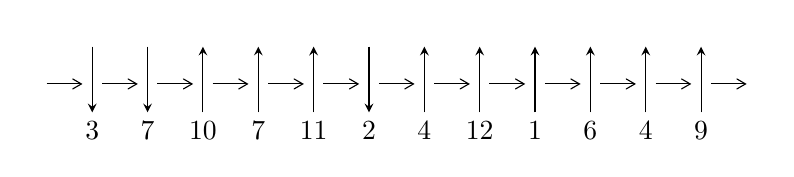
\begin{tikzpicture}[x=20pt, y=17pt]
	% nodes
	\node (C0) at (0, 0) {};
	\node (C1) at (1, 0) {};
	\node (C1U) at (1, +1) {};
	\node (C1D) at (1, -1) {3};

	\node (C2) at (2, 0) {};
	\node (C2U) at (2, +1) {};
	\node (C2D) at (2, -1) {7};

	\node (C3) at (3, 0) {};
	\node (C3U) at (3, +1) {};
	\node (C3D) at (3, -1) {10};

	\node (C4) at (4, 0) {};
	\node (C4U) at (4, +1) {};
	\node (C4D) at (4, -1) {7};

	\node (C5) at (5, 0) {};
	\node (C5U) at (5, +1) {};
	\node (C5D) at (5, -1) {11};

	\node (C6) at (6, 0) {};
	\node (C6U) at (6, +1) {};
	\node (C6D) at (6, -1) {2};

	\node (C7) at (7, 0) {};
	\node (C7U) at (7, +1) {};
	\node (C7D) at (7, -1) {4};

	\node (C8) at (8, 0) {};
	\node (C8U) at (8, +1) {};
	\node (C8D) at (8, -1) {12};

	\node (C9) at (9, 0) {};
	\node (C9U) at (9, +1) {};
	\node (C9D) at (9, -1) {1};

	\node (C10) at (10, 0) {};
	\node (C10U) at (10, +1) {};
	\node (C10D) at (10, -1) {6};

	\node (C11) at (11, 0) {};
	\node (C11U) at (11, +1) {};
	\node (C11D) at (11, -1) {4};

	\node (C12) at (12, 0) {};
	\node (C12U) at (12, +1) {};
	\node (C12D) at (12, -1) {9};
	\node (C13) at (13, 0) {};

	% arrows
	\draw[->,>={angle 60}]
	(C0) edge (C1) (C1) edge (C2) (C2) edge (C3) (C3) edge (C4) (C4) edge (C5) (C5) edge (C6) (C6) edge (C7) (C7) edge (C8) (C8) edge (C9) (C9) edge (C10) (C10) edge (C11) (C11) edge (C12) (C12) edge (C13) ;	\draw[->,>=stealth]
	(C1U) edge (C1D) (C2U) edge (C2D) (C3D) edge (C3U) (C4D) edge (C4U) (C5D) edge (C5U) (C6U) edge (C6D) (C7D) edge (C7U) (C8D) edge (C8U) (C9D) edge (C9U) (C10D) edge (C10U) (C11D) edge (C11U) (C12D) edge (C12U) ;
	\end{tikzpicture} \\
\hhline{~~} \\& 
\textbf{Solving Sequence} \\ \cline{2-2} 
 &
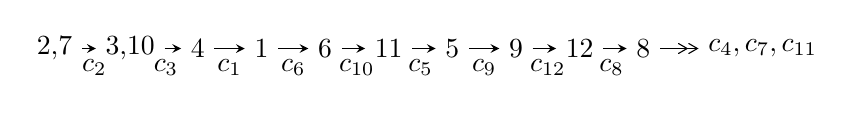
\begin{tikzpicture}[x=23pt, y=7pt]
	% node
	\node (A0) at (-1/8, 0) {2,7};
	\node (A1) at (17/16, 0) {3,10};
	\node (A2) at (17/8, 0) {4};
	\node (A3) at (25/8, 0) {1};
	\node (A4) at (33/8, 0) {6};
	\node (A5) at (41/8, 0) {11};
	\node (A6) at (49/8, 0) {5};
	\node (A7) at (57/8, 0) {9};
	\node (A8) at (65/8, 0) {12};
	\node (A9) at (73/8, 0) {8};
	\node (C1) at (1/2, -1) {$c_{2}$};
	\node (C2) at (13/8, -1) {$c_{3}$};
	\node (C3) at (21/8, -1) {$c_{1}$};
	\node (C4) at (29/8, -1) {$c_{6}$};
	\node (C5) at (37/8, -1) {$c_{10}$};
	\node (C6) at (45/8, -1) {$c_{5}$};
	\node (C7) at (53/8, -1) {$c_{9}$};
	\node (C8) at (61/8, -1) {$c_{12}$};
	\node (C9) at (69/8, -1) {$c_{8}$};
	\node (A10) at (11, 0) {$c_{4},c_{7},c_{11}$};

	% edge
	\draw[->,>=stealth]	
	(A0) edge (A1) (A1) edge (A2) (A2) edge (A3) (A3) edge (A4) (A4) edge (A5) (A5) edge (A6) (A6) edge (A7) (A7) edge (A8) (A8) edge (A9) ;
	\draw[->>,>={angle 60}]	
	(A9) edge (A10);
\end{tikzpicture} \\ 

\end{tabular} \\

\footnotetext{
The image of knot diagram is generated by the software ``\textbf{Draw programme}" developed by Andrew Bartholomew(\url{http://www.layer8.co.uk/maths/draw/index.htm\#Running-draw}), where we modified some parts for our purpose(\url{https://github.com/CATsTAILs/LinksPainter}).
}\phantom \\ \newline 
\centering \textbf{Ideals for irreducible components\footnotemark of $X_{\text{par}}$} 
 
\begin{align*}
I^u_{1}&=\langle 
-13 u^{16}-54 u^{15}+\cdots+4 b-36,\;-9 u^{16}-28 u^{15}+\cdots+8 a+20,\;u^{17}+6 u^{16}+\cdots+56 u+8\rangle \\
I^u_{2}&=\langle 
3 u^{10}-8 u^9+3 u^8+16 u^7-11 u^6-21 u^5+21 u^4+16 u^3-17 u^2+b-6 u+6,\\
\phantom{I^u_{2}}&\phantom{= \langle  }6 u^{10}-15 u^9+4 u^8+33 u^7-20 u^6-41 u^5+39 u^4+33 u^3-32 u^2+a-11 u+12,\\
\phantom{I^u_{2}}&\phantom{= \langle  }u^{11}-3 u^{10}+2 u^9+5 u^8-6 u^7-5 u^6+10 u^5+2 u^4-8 u^3+u^2+3 u-1\rangle \\
I^u_{3}&=\langle 
-37 a^5 u^2+123 a^4 u^2+\cdots-100 a+168,\;a^5 u^2-3 a^4 u^2+\cdots+13 a+20,\;u^3- u^2+1\rangle \\
\\
\end{align*}
\raggedright * 3 irreducible components of $\dim_{\mathbb{C}}=0$, with total 46 representations.\\
\footnotetext{All coefficients of polynomials are rational numbers. But the coefficients are sometimes approximated in decimal forms when there is not enough margin.}
\newpage
\renewcommand{\arraystretch}{1}
\centering \section*{I. $I^u_{1}= \langle -13 u^{16}-54 u^{15}+\cdots+4 b-36,\;-9 u^{16}-28 u^{15}+\cdots+8 a+20,\;u^{17}+6 u^{16}+\cdots+56 u+8 \rangle$}
\flushleft \textbf{(i) Arc colorings}\\
\begin{tabular}{m{7pt} m{180pt} m{7pt} m{180pt} }
\flushright $a_{2}=$&$\begin{pmatrix}1\\0\end{pmatrix}$ \\
\flushright $a_{7}=$&$\begin{pmatrix}0\\u\end{pmatrix}$ \\
\flushright $a_{3}=$&$\begin{pmatrix}1\\u^2\end{pmatrix}$ \\
\flushright $a_{10}=$&$\begin{pmatrix}\frac{9}{8} u^{16}+\frac{7}{2} u^{15}+\cdots-\frac{29}{2} u-\frac{5}{2}\\\frac{13}{4} u^{16}+\frac{27}{2} u^{15}+\cdots+\frac{131}{2} u+9\end{pmatrix}$ \\
\flushright $a_{4}=$&$\begin{pmatrix}\frac{1}{4} u^{16}+u^{15}+\cdots+\frac{3}{2} u+\frac{1}{2}\\\frac{1}{2} u^{16}+\frac{5}{2} u^{15}+\cdots+\frac{29}{2} u+2\end{pmatrix}$ \\
\flushright $a_{1}=$&$\begin{pmatrix}- u^2+1\\- u^4\end{pmatrix}$ \\
\flushright $a_{6}=$&$\begin{pmatrix}u\\u\end{pmatrix}$ \\
\flushright $a_{11}=$&$\begin{pmatrix}\frac{33}{8} u^{16}+\frac{39}{2} u^{15}+\cdots+\frac{245}{2} u+\frac{39}{2}\\\frac{25}{4} u^{16}+\frac{59}{2} u^{15}+\cdots+\frac{405}{2} u+31\end{pmatrix}$ \\
\flushright $a_{5}=$&$\begin{pmatrix}\frac{1}{4} u^{16}+u^{15}+\cdots+\frac{3}{2} u+\frac{1}{2}\\-\frac{1}{2} u^{15}-2 u^{14}+\cdots-\frac{23}{2} u-2\end{pmatrix}$ \\
\flushright $a_{9}=$&$\begin{pmatrix}-\frac{9}{8} u^{16}-4 u^{15}+\cdots+12 u+\frac{9}{2}\\-\frac{15}{4} u^{16}-\frac{29}{2} u^{15}+\cdots-\frac{29}{2} u+1\end{pmatrix}$ \\
\flushright $a_{12}=$&$\begin{pmatrix}\frac{9}{4} u^{16}+12 u^{15}+\cdots+\frac{201}{2} u+\frac{35}{2}\\2 u^{16}+\frac{25}{2} u^{15}+\cdots+\frac{311}{2} u+26\end{pmatrix}$ \\
\flushright $a_{8}=$&$\begin{pmatrix}-\frac{11}{4} u^{16}-\frac{59}{4} u^{15}+\cdots-\frac{429}{4} u-16\\-\frac{9}{4} u^{16}-14 u^{15}+\cdots-141 u-22\end{pmatrix}$\\&\end{tabular}
\flushleft \textbf{(ii) Obstruction class $= -1$}\\~\\
\flushleft \textbf{(iii) Cusp Shapes $= -9 u^{16}-52 u^{15}-116 u^{14}-68 u^{13}+190 u^{12}+347 u^{11}-140 u^{10}-1029 u^9-1025 u^8+472 u^7+1947 u^6+1504 u^5-415 u^4-1702 u^3-1433 u^2-576 u-82$}\\~\\
\newpage\renewcommand{\arraystretch}{1}
\flushleft \textbf{(iv) u-Polynomials at the component}\newline \\
\begin{tabular}{m{50pt}|m{274pt}}
Crossings & \hspace{64pt}u-Polynomials at each crossing \\
\hline $$\begin{aligned}c_{1}\end{aligned}$$&$\begin{aligned}
&u^{17}+6 u^{16}+\cdots+480 u+64
\end{aligned}$\\
\hline $$\begin{aligned}c_{2},c_{6}\end{aligned}$$&$\begin{aligned}
&u^{17}-6 u^{16}+\cdots+56 u-8
\end{aligned}$\\
\hline $$\begin{aligned}c_{3},c_{5},c_{10}\end{aligned}$$&$\begin{aligned}
&u^{17}- u^{15}+\cdots+3 u-1
\end{aligned}$\\
\hline $$\begin{aligned}c_{4},c_{7}\end{aligned}$$&$\begin{aligned}
&u^{17}+4 u^{16}+\cdots+8 u-1
\end{aligned}$\\
\hline $$\begin{aligned}c_{8},c_{9},c_{12}\end{aligned}$$&$\begin{aligned}
&u^{17}-7 u^{16}+\cdots+20 u-8
\end{aligned}$\\
\hline $$\begin{aligned}c_{11}\end{aligned}$$&$\begin{aligned}
&u^{17}-2 u^{16}+\cdots+u-1
\end{aligned}$\\
\hline
\end{tabular}\\~\\
\newpage\renewcommand{\arraystretch}{1}
\flushleft \textbf{(v) Riley Polynomials at the component}\newline \\
\begin{tabular}{m{50pt}|m{274pt}}
Crossings & \hspace{64pt}Riley Polynomials at each crossing \\
\hline $$\begin{aligned}c_{1}\end{aligned}$$&$\begin{aligned}
&y^{17}+22 y^{16}+\cdots+66048 y-4096
\end{aligned}$\\
\hline $$\begin{aligned}c_{2},c_{6}\end{aligned}$$&$\begin{aligned}
&y^{17}-6 y^{16}+\cdots+480 y-64
\end{aligned}$\\
\hline $$\begin{aligned}c_{3},c_{5},c_{10}\end{aligned}$$&$\begin{aligned}
&y^{17}-2 y^{16}+\cdots+3 y-1
\end{aligned}$\\
\hline $$\begin{aligned}c_{4},c_{7}\end{aligned}$$&$\begin{aligned}
&y^{17}-36 y^{16}+\cdots+102 y-1
\end{aligned}$\\
\hline $$\begin{aligned}c_{8},c_{9},c_{12}\end{aligned}$$&$\begin{aligned}
&y^{17}-21 y^{16}+\cdots+272 y-64
\end{aligned}$\\
\hline $$\begin{aligned}c_{11}\end{aligned}$$&$\begin{aligned}
&y^{17}-44 y^{16}+\cdots+33 y-1
\end{aligned}$\\
\hline
\end{tabular}\\~\\
\newpage\flushleft \textbf{(vi) Complex Volumes and Cusp Shapes}
$$\begin{array}{c|c|c}  
\text{Solutions to }I^u_{1}& \I (\text{vol} + \sqrt{-1}CS) & \text{Cusp shape}\\
 \hline 
\begin{aligned}
u &= -0.582631 + 0.962982 I \\
a &= -0.764828 + 0.649431 I \\
b &= \phantom{-}0.179778 + 1.114890 I\end{aligned}
 & \phantom{-}6.08323 - 3.07842 I & \phantom{-}10.91849 + 3.36026 I \\ \hline\begin{aligned}
u &= -0.582631 - 0.962982 I \\
a &= -0.764828 - 0.649431 I \\
b &= \phantom{-}0.179778 - 1.114890 I\end{aligned}
 & \phantom{-}6.08323 + 3.07842 I & \phantom{-}10.91849 - 3.36026 I \\ \hline\begin{aligned}
u &= -0.998116 + 0.574654 I \\
a &= -1.30029 + 0.75173 I \\
b &= -0.86585 + 1.49753 I\end{aligned}
 & -0.04390 + 4.58131 I & \phantom{-}7.64977 - 6.92778 I \\ \hline\begin{aligned}
u &= -0.998116 - 0.574654 I \\
a &= -1.30029 - 0.75173 I \\
b &= -0.86585 - 1.49753 I\end{aligned}
 & -0.04390 - 4.58131 I & \phantom{-}7.64977 + 6.92778 I \\ \hline\begin{aligned}
u &= \phantom{-}1.139290 + 0.263587 I \\
a &= \phantom{-}0.072389 + 0.255610 I \\
b &= -0.015097 - 0.310294 I\end{aligned}
 & -2.02646 - 1.69138 I & \phantom{-}0.73300 + 3.24851 I \\ \hline\begin{aligned}
u &= \phantom{-}1.139290 - 0.263587 I \\
a &= \phantom{-}0.072389 - 0.255610 I \\
b &= -0.015097 + 0.310294 I\end{aligned}
 & -2.02646 + 1.69138 I & \phantom{-}0.73300 - 3.24851 I \\ \hline\begin{aligned}
u &= -0.612038 + 0.494740 I \\
a &= \phantom{-}1.36351 - 0.44192 I \\
b &= \phantom{-}0.615883 - 0.945055 I\end{aligned}
 & \phantom{-}1.133960 - 0.080801 I & \phantom{-}10.62347 + 1.71983 I \\ \hline\begin{aligned}
u &= -0.612038 - 0.494740 I \\
a &= \phantom{-}1.36351 + 0.44192 I \\
b &= \phantom{-}0.615883 + 0.945055 I\end{aligned}
 & \phantom{-}1.133960 + 0.080801 I & \phantom{-}10.62347 - 1.71983 I \\ \hline\begin{aligned}
u &= -0.710496 + 1.098260 I \\
a &= \phantom{-}0.517258 - 0.878567 I \\
b &= -0.597387 - 1.192300 I\end{aligned}
 & \phantom{-}16.3616 - 5.2854 I & \phantom{-}10.20532 + 2.53472 I \\ \hline\begin{aligned}
u &= -0.710496 - 1.098260 I \\
a &= \phantom{-}0.517258 + 0.878567 I \\
b &= -0.597387 + 1.192300 I\end{aligned}
 & \phantom{-}16.3616 + 5.2854 I & \phantom{-}10.20532 - 2.53472 I\\
 \hline 
 \end{array}$$\newpage$$\begin{array}{c|c|c}  
\text{Solutions to }I^u_{1}& \I (\text{vol} + \sqrt{-1}CS) & \text{Cusp shape}\\
 \hline 
\begin{aligned}
u &= -1.105090 + 0.729938 I \\
a &= \phantom{-}1.30956 - 0.56888 I \\
b &= \phantom{-}1.03194 - 1.58456 I\end{aligned}
 & \phantom{-}4.45386 + 9.24930 I & \phantom{-}8.34005 - 7.37887 I \\ \hline\begin{aligned}
u &= -1.105090 - 0.729938 I \\
a &= \phantom{-}1.30956 + 0.56888 I \\
b &= \phantom{-}1.03194 + 1.58456 I\end{aligned}
 & \phantom{-}4.45386 - 9.24930 I & \phantom{-}8.34005 + 7.37887 I \\ \hline\begin{aligned}
u &= -1.126030 + 0.831805 I \\
a &= -1.43522 + 0.37456 I \\
b &= -1.30455 + 1.61559 I\end{aligned}
 & \phantom{-}14.9808 + 12.2193 I & \phantom{-}8.76311 - 5.87051 I \\ \hline\begin{aligned}
u &= -1.126030 - 0.831805 I \\
a &= -1.43522 - 0.37456 I \\
b &= -1.30455 - 1.61559 I\end{aligned}
 & \phantom{-}14.9808 - 12.2193 I & \phantom{-}8.76311 + 5.87051 I \\ \hline\begin{aligned}
u &= \phantom{-}1.22314 + 0.77434 I \\
a &= -0.144243 - 0.159249 I \\
b &= \phantom{-}0.053117 + 0.306476 I\end{aligned}
 & \phantom{-}4.66481 - 3.72406 I & \phantom{-}7.31637 - 0.66089 I \\ \hline\begin{aligned}
u &= \phantom{-}1.22314 - 0.77434 I \\
a &= -0.144243 + 0.159249 I \\
b &= \phantom{-}0.053117 - 0.306476 I\end{aligned}
 & \phantom{-}4.66481 + 3.72406 I & \phantom{-}7.31637 + 0.66089 I \\ \hline\begin{aligned}
u &= -0.456042\phantom{ +0.000000I} \\
a &= \phantom{-}1.76372\phantom{ +0.000000I} \\
b &= \phantom{-}0.804333\phantom{ +0.000000I}\end{aligned}
 & \phantom{-}0.900511\phantom{ +0.000000I} & \phantom{-}10.9010\phantom{ +0.000000I}\\
 \hline 
 \end{array}$$\newpage\newpage\renewcommand{\arraystretch}{1}
\centering \section*{II. $I^u_{2}= \langle 3 u^{10}-8 u^9+\cdots+b+6,\;6 u^{10}-15 u^9+\cdots+a+12,\;u^{11}-3 u^{10}+\cdots+3 u-1 \rangle$}
\flushleft \textbf{(i) Arc colorings}\\
\begin{tabular}{m{7pt} m{180pt} m{7pt} m{180pt} }
\flushright $a_{2}=$&$\begin{pmatrix}1\\0\end{pmatrix}$ \\
\flushright $a_{7}=$&$\begin{pmatrix}0\\u\end{pmatrix}$ \\
\flushright $a_{3}=$&$\begin{pmatrix}1\\u^2\end{pmatrix}$ \\
\flushright $a_{10}=$&$\begin{pmatrix}-6 u^{10}+15 u^9+\cdots+11 u-12\\-3 u^{10}+8 u^9+\cdots+6 u-6\end{pmatrix}$ \\
\flushright $a_{4}=$&$\begin{pmatrix}-3 u^{10}+8 u^9+\cdots+5 u-9\\- u^{10}+3 u^9-2 u^8-5 u^7+6 u^6+5 u^5-10 u^4-2 u^3+9 u^2- u-3\end{pmatrix}$ \\
\flushright $a_{1}=$&$\begin{pmatrix}- u^2+1\\- u^4\end{pmatrix}$ \\
\flushright $a_{6}=$&$\begin{pmatrix}u\\u\end{pmatrix}$ \\
\flushright $a_{11}=$&$\begin{pmatrix}-5 u^{10}+13 u^9+\cdots+8 u-10\\-2 u^{10}+6 u^9-4 u^8-9 u^7+9 u^6+12 u^5-16 u^4-8 u^3+12 u^2+3 u-4\end{pmatrix}$ \\
\flushright $a_{5}=$&$\begin{pmatrix}-3 u^{10}+8 u^9+\cdots+5 u-9\\- u^{10}+3 u^9-2 u^8-5 u^7+6 u^6+5 u^5-10 u^4-2 u^3+8 u^2- u-2\end{pmatrix}$ \\
\flushright $a_{9}=$&$\begin{pmatrix}-4 u^{10}+10 u^9+\cdots+7 u-8\\-3 u^{10}+8 u^9+\cdots+6 u-6\end{pmatrix}$ \\
\flushright $a_{12}=$&$\begin{pmatrix}4 u^{10}-10 u^9+\cdots-4 u+11\\3 u^{10}-7 u^9+u^8+16 u^7-8 u^6-19 u^5+17 u^4+14 u^3-13 u^2-3 u+6\end{pmatrix}$ \\
\flushright $a_{8}=$&$\begin{pmatrix}8 u^{10}-21 u^9+\cdots-13 u+19\\3 u^{10}-8 u^9+\cdots-5 u+9\end{pmatrix}$\\&\end{tabular}
\flushleft \textbf{(ii) Obstruction class $= 1$}\\~\\
\flushleft \textbf{(iii) Cusp Shapes $= 7 u^{10}-19 u^9+13 u^8+28 u^7-27 u^6-29 u^5+51 u^4+18 u^3-28 u^2+u+16$}\\~\\
\newpage\renewcommand{\arraystretch}{1}
\flushleft \textbf{(iv) u-Polynomials at the component}\newline \\
\begin{tabular}{m{50pt}|m{274pt}}
Crossings & \hspace{64pt}u-Polynomials at each crossing \\
\hline $$\begin{aligned}c_{1}\end{aligned}$$&$\begin{aligned}
&u^{11}-5 u^{10}+\cdots+11 u-1
\end{aligned}$\\
\hline $$\begin{aligned}c_{2}\end{aligned}$$&$\begin{aligned}
&u^{11}-3 u^{10}+2 u^9+5 u^8-6 u^7-5 u^6+10 u^5+2 u^4-8 u^3+u^2+3 u-1
\end{aligned}$\\
\hline $$\begin{aligned}c_{3},c_{10}\end{aligned}$$&$\begin{aligned}
&u^{11}+4 u^9+u^8+4 u^7+4 u^6- u^5+5 u^4-2 u^3+3 u^2- u+1
\end{aligned}$\\
\hline $$\begin{aligned}c_{4}\end{aligned}$$&$\begin{aligned}
&u^{11}+3 u^9+6 u^8+u^7+20 u^6-4 u^5+26 u^4-6 u^3+15 u^2-4 u+3
\end{aligned}$\\
\hline $$\begin{aligned}c_{5}\end{aligned}$$&$\begin{aligned}
&u^{11}+4 u^9- u^8+4 u^7-4 u^6- u^5-5 u^4-2 u^3-3 u^2- u-1
\end{aligned}$\\
\hline $$\begin{aligned}c_{6}\end{aligned}$$&$\begin{aligned}
&u^{11}+3 u^{10}+2 u^9-5 u^8-6 u^7+5 u^6+10 u^5-2 u^4-8 u^3- u^2+3 u+1
\end{aligned}$\\
\hline $$\begin{aligned}c_{7}\end{aligned}$$&$\begin{aligned}
&u^{11}+3 u^9-6 u^8+u^7-20 u^6-4 u^5-26 u^4-6 u^3-15 u^2-4 u-3
\end{aligned}$\\
\hline $$\begin{aligned}c_{8},c_{9}\end{aligned}$$&$\begin{aligned}
&u^{11}-8 u^9- u^8+23 u^7+5 u^6-28 u^5-7 u^4+13 u^3+2 u^2-2 u-1
\end{aligned}$\\
\hline $$\begin{aligned}c_{11}\end{aligned}$$&$\begin{aligned}
&u^{11}+7 u^9-22 u^8+7 u^7-56 u^6-3 u^5-45 u^4-6 u^3-12 u^2- u-1
\end{aligned}$\\
\hline $$\begin{aligned}c_{12}\end{aligned}$$&$\begin{aligned}
&u^{11}-8 u^9+u^8+23 u^7-5 u^6-28 u^5+7 u^4+13 u^3-2 u^2-2 u+1
\end{aligned}$\\
\hline
\end{tabular}\\~\\
\newpage\renewcommand{\arraystretch}{1}
\flushleft \textbf{(v) Riley Polynomials at the component}\newline \\
\begin{tabular}{m{50pt}|m{274pt}}
Crossings & \hspace{64pt}Riley Polynomials at each crossing \\
\hline $$\begin{aligned}c_{1}\end{aligned}$$&$\begin{aligned}
&y^{11}+19 y^{10}+\cdots+31 y-1
\end{aligned}$\\
\hline $$\begin{aligned}c_{2},c_{6}\end{aligned}$$&$\begin{aligned}
&y^{11}-5 y^{10}+\cdots+11 y-1
\end{aligned}$\\
\hline $$\begin{aligned}c_{3},c_{5},c_{10}\end{aligned}$$&$\begin{aligned}
&y^{11}+8 y^{10}+\cdots-5 y-1
\end{aligned}$\\
\hline $$\begin{aligned}c_{4},c_{7}\end{aligned}$$&$\begin{aligned}
&y^{11}+6 y^{10}+\cdots-74 y-9
\end{aligned}$\\
\hline $$\begin{aligned}c_{8},c_{9},c_{12}\end{aligned}$$&$\begin{aligned}
&y^{11}-16 y^{10}+\cdots+8 y-1
\end{aligned}$\\
\hline $$\begin{aligned}c_{11}\end{aligned}$$&$\begin{aligned}
&y^{11}+14 y^{10}+\cdots-23 y-1
\end{aligned}$\\
\hline
\end{tabular}\\~\\
\newpage\flushleft \textbf{(vi) Complex Volumes and Cusp Shapes}
$$\begin{array}{c|c|c}  
\text{Solutions to }I^u_{2}& \I (\text{vol} + \sqrt{-1}CS) & \text{Cusp shape}\\
 \hline 
\begin{aligned}
u &= -0.856562 + 0.586236 I \\
a &= -0.588949 + 0.335331 I \\
b &= \phantom{-}0.307889 - 0.632495 I\end{aligned}
 & \phantom{-}2.23625 + 2.32410 I & \phantom{-}6.78884 - 2.44901 I \\ \hline\begin{aligned}
u &= -0.856562 - 0.586236 I \\
a &= -0.588949 - 0.335331 I \\
b &= \phantom{-}0.307889 + 0.632495 I\end{aligned}
 & \phantom{-}2.23625 - 2.32410 I & \phantom{-}6.78884 + 2.44901 I \\ \hline\begin{aligned}
u &= -0.855558 + 0.209235 I \\
a &= \phantom{-}0.357696 - 0.809834 I \\
b &= -0.136583 + 0.767702 I\end{aligned}
 & -5.34223 + 0.90366 I & \phantom{-}2.99552 - 7.97302 I \\ \hline\begin{aligned}
u &= -0.855558 - 0.209235 I \\
a &= \phantom{-}0.357696 + 0.809834 I \\
b &= -0.136583 - 0.767702 I\end{aligned}
 & -5.34223 - 0.90366 I & \phantom{-}2.99552 + 7.97302 I \\ \hline\begin{aligned}
u &= \phantom{-}0.736045 + 0.353997 I \\
a &= \phantom{-}1.99508 - 0.41979 I \\
b &= \phantom{-}1.61707 + 0.39727 I\end{aligned}
 & \phantom{-}0.857139 - 1.116710 I & \phantom{-}8.63274 + 6.10960 I \\ \hline\begin{aligned}
u &= \phantom{-}0.736045 - 0.353997 I \\
a &= \phantom{-}1.99508 + 0.41979 I \\
b &= \phantom{-}1.61707 - 0.39727 I\end{aligned}
 & \phantom{-}0.857139 + 1.116710 I & \phantom{-}8.63274 - 6.10960 I \\ \hline\begin{aligned}
u &= \phantom{-}1.011880 + 0.753500 I \\
a &= -0.801625 + 0.134986 I \\
b &= -0.912860 - 0.467435 I\end{aligned}
 & -1.90477 - 3.17083 I & -2.15194 + 8.40607 I \\ \hline\begin{aligned}
u &= \phantom{-}1.011880 - 0.753500 I \\
a &= -0.801625 - 0.134986 I \\
b &= -0.912860 + 0.467435 I\end{aligned}
 & -1.90477 + 3.17083 I & -2.15194 - 8.40607 I \\ \hline\begin{aligned}
u &= \phantom{-}0.419548\phantom{ +0.000000I} \\
a &= -4.82997\phantom{ +0.000000I} \\
b &= -2.02640\phantom{ +0.000000I}\end{aligned}
 & \phantom{-}12.4935\phantom{ +0.000000I} & \phantom{-}13.9460\phantom{ +0.000000I} \\ \hline\begin{aligned}
u &= \phantom{-}1.25442 + 1.05470 I \\
a &= \phantom{-}0.452785 - 0.066086 I \\
b &= \phantom{-}0.637684 + 0.394653 I\end{aligned}
 & \phantom{-}4.48658 - 4.37367 I & \phantom{-}3.76171 + 10.00302 I\\
 \hline 
 \end{array}$$\newpage$$\begin{array}{c|c|c}  
\text{Solutions to }I^u_{2}& \I (\text{vol} + \sqrt{-1}CS) & \text{Cusp shape}\\
 \hline 
\begin{aligned}
u &= \phantom{-}1.25442 - 1.05470 I \\
a &= \phantom{-}0.452785 + 0.066086 I \\
b &= \phantom{-}0.637684 - 0.394653 I\end{aligned}
 & \phantom{-}4.48658 + 4.37367 I & \phantom{-}3.76171 - 10.00302 I\\
 \hline 
 \end{array}$$\newpage\newpage\renewcommand{\arraystretch}{1}
\centering \section*{III. $I^u_{3}= \langle -37 a^5 u^2+123 a^4 u^2+\cdots-100 a+168,\;a^5 u^2-3 a^4 u^2+\cdots+13 a+20,\;u^3- u^2+1 \rangle$}
\flushleft \textbf{(i) Arc colorings}\\
\begin{tabular}{m{7pt} m{180pt} m{7pt} m{180pt} }
\flushright $a_{2}=$&$\begin{pmatrix}1\\0\end{pmatrix}$ \\
\flushright $a_{7}=$&$\begin{pmatrix}0\\u\end{pmatrix}$ \\
\flushright $a_{3}=$&$\begin{pmatrix}1\\u^2\end{pmatrix}$ \\
\flushright $a_{10}=$&$\begin{pmatrix}a\\0.110778 a^{5} u^{2}-0.368263 a^{4} u^{2}+\cdots+0.299401 a-0.502994\end{pmatrix}$ \\
\flushright $a_{4}=$&$\begin{pmatrix}0.182635 a^{5} u^{2}-0.323353 a^{4} u^{2}+\cdots-0.371257 a+0.143713\\0.365269 a^{5} u^{2}-0.646707 a^{4} u^{2}+\cdots-0.742515 a+0.287425\end{pmatrix}$ \\
\flushright $a_{1}=$&$\begin{pmatrix}- u^2+1\\- u^2+u+1\end{pmatrix}$ \\
\flushright $a_{6}=$&$\begin{pmatrix}u\\u\end{pmatrix}$ \\
\flushright $a_{11}=$&$\begin{pmatrix}0.434132 a^{5} u^{2}+0.0838323 a^{4} u^{2}+\cdots-0.718563 a-0.592814\\0.544910 a^{5} u^{2}-0.284431 a^{4} u^{2}+\cdots-1.41916 a-1.09581\end{pmatrix}$ \\
\flushright $a_{5}=$&$\begin{pmatrix}0.182635 a^{5} u^{2}-0.323353 a^{4} u^{2}+\cdots-0.371257 a+0.143713\\0.703593 a^{5} u^{2}-1.12275 a^{4} u^{2}+\cdots-0.733533 a+0.832335\end{pmatrix}$ \\
\flushright $a_{9}=$&$\begin{pmatrix}0.799401 a^{5} u^{2}-0.0628743 a^{4} u^{2}+\cdots-0.461078 a-0.305389\\0.868263 a^{5} u^{2}+0.167665 a^{4} u^{2}+\cdots-1.43713 a-1.18563\end{pmatrix}$ \\
\flushright $a_{12}=$&$\begin{pmatrix}-1.00898 a^{5} u^{2}+1.55689 a^{4} u^{2}+\cdots+0.583832 a-0.580838\\-0.853293 a^{5} u^{2}+1.40419 a^{4} u^{2}+\cdots+0.964072 a-0.179641\end{pmatrix}$ \\
\flushright $a_{8}=$&$\begin{pmatrix}-0.407186 a^{5} u^{2}+1.24551 a^{4} u^{2}+\cdots+0.467066 a-0.664671\\-0.736527 a^{5} u^{2}+1.66467 a^{4} u^{2}+\cdots+0.874251 a-0.628743\end{pmatrix}$\\&\end{tabular}
\flushleft \textbf{(ii) Obstruction class $= -1$}\\~\\
\flushleft \textbf{(iii) Cusp Shapes $= 4 u+6$}\\~\\
\newpage\renewcommand{\arraystretch}{1}
\flushleft \textbf{(iv) u-Polynomials at the component}\newline \\
\begin{tabular}{m{50pt}|m{274pt}}
Crossings & \hspace{64pt}u-Polynomials at each crossing \\
\hline $$\begin{aligned}c_{1}\end{aligned}$$&$\begin{aligned}
&(u^3+u^2+2 u+1)^6
\end{aligned}$\\
\hline $$\begin{aligned}c_{2},c_{6}\end{aligned}$$&$\begin{aligned}
&(u^3+u^2-1)^6
\end{aligned}$\\
\hline $$\begin{aligned}c_{3},c_{5},c_{10}\end{aligned}$$&$\begin{aligned}
&u^{18}+u^{17}+\cdots+4 u-8
\end{aligned}$\\
\hline $$\begin{aligned}c_{4},c_{7}\end{aligned}$$&$\begin{aligned}
&u^{18}+u^{17}+\cdots-684 u-216
\end{aligned}$\\
\hline $$\begin{aligned}c_{8},c_{9},c_{12}\end{aligned}$$&$\begin{aligned}
&(u^3+u^2-2 u-1)^6
\end{aligned}$\\
\hline $$\begin{aligned}c_{11}\end{aligned}$$&$\begin{aligned}
&u^{18}- u^{17}+\cdots-196 u-392
\end{aligned}$\\
\hline
\end{tabular}\\~\\
\newpage\renewcommand{\arraystretch}{1}
\flushleft \textbf{(v) Riley Polynomials at the component}\newline \\
\begin{tabular}{m{50pt}|m{274pt}}
Crossings & \hspace{64pt}Riley Polynomials at each crossing \\
\hline $$\begin{aligned}c_{1}\end{aligned}$$&$\begin{aligned}
&(y^3+3 y^2+2 y-1)^6
\end{aligned}$\\
\hline $$\begin{aligned}c_{2},c_{6}\end{aligned}$$&$\begin{aligned}
&(y^3- y^2+2 y-1)^6
\end{aligned}$\\
\hline $$\begin{aligned}c_{3},c_{5},c_{10}\end{aligned}$$&$\begin{aligned}
&y^{18}+3 y^{17}+\cdots-80 y+64
\end{aligned}$\\
\hline $$\begin{aligned}c_{4},c_{7}\end{aligned}$$&$\begin{aligned}
&y^{18}-21 y^{17}+\cdots+55728 y+46656
\end{aligned}$\\
\hline $$\begin{aligned}c_{8},c_{9},c_{12}\end{aligned}$$&$\begin{aligned}
&(y^3-5 y^2+6 y-1)^6
\end{aligned}$\\
\hline $$\begin{aligned}c_{11}\end{aligned}$$&$\begin{aligned}
&y^{18}-33 y^{17}+\cdots-16464 y+153664
\end{aligned}$\\
\hline
\end{tabular}\\~\\
\newpage\flushleft \textbf{(vi) Complex Volumes and Cusp Shapes}
$$\begin{array}{c|c|c}  
\text{Solutions to }I^u_{3}& \I (\text{vol} + \sqrt{-1}CS) & \text{Cusp shape}\\
 \hline 
\begin{aligned}
u &= \phantom{-}0.877439 + 0.744862 I \\
a &= \phantom{-}0.961970 - 0.199906 I \\
b &= \phantom{-}0.842708 + 0.290892 I\end{aligned}
 & -1.20570 - 2.82812 I & \phantom{-}9.50976 + 2.97945 I \\ \hline\begin{aligned}
u &= \phantom{-}0.877439 + 0.744862 I \\
a &= -0.641730 - 0.729183 I \\
b &= -0.62835 - 2.13101 I\end{aligned}
 & \phantom{-}15.7136 - 2.8281 I & \phantom{-}9.50976 + 2.97945 I \\ \hline\begin{aligned}
u &= \phantom{-}0.877439 + 0.744862 I \\
a &= -0.721738 + 0.281163 I \\
b &= -0.992973 - 0.541129 I\end{aligned}
 & -1.20570 - 2.82812 I & \phantom{-}9.50976 + 2.97945 I \\ \hline\begin{aligned}
u &= \phantom{-}0.877439 + 0.744862 I \\
a &= -1.189520 - 0.508099 I \\
b &= -0.244232 - 0.630700 I\end{aligned}
 & \phantom{-}4.43407 - 2.82812 I & \phantom{-}9.50976 + 2.97945 I \\ \hline\begin{aligned}
u &= \phantom{-}0.877439 + 0.744862 I \\
a &= \phantom{-}0.516399 + 0.280423 I \\
b &= \phantom{-}0.66526 + 1.33185 I\end{aligned}
 & \phantom{-}4.43407 - 2.82812 I & \phantom{-}9.50976 + 2.97945 I \\ \hline\begin{aligned}
u &= \phantom{-}0.877439 + 0.744862 I \\
a &= \phantom{-}1.61441 + 1.05819 I \\
b &= \phantom{-}0.019938 + 1.117810 I\end{aligned}
 & \phantom{-}15.7136 - 2.8281 I & \phantom{-}9.50976 + 2.97945 I \\ \hline\begin{aligned}
u &= \phantom{-}0.877439 - 0.744862 I \\
a &= \phantom{-}0.961970 + 0.199906 I \\
b &= \phantom{-}0.842708 - 0.290892 I\end{aligned}
 & -1.20570 + 2.82812 I & \phantom{-}9.50976 - 2.97945 I \\ \hline\begin{aligned}
u &= \phantom{-}0.877439 - 0.744862 I \\
a &= -0.641730 + 0.729183 I \\
b &= -0.62835 + 2.13101 I\end{aligned}
 & \phantom{-}15.7136 + 2.8281 I & \phantom{-}9.50976 - 2.97945 I \\ \hline\begin{aligned}
u &= \phantom{-}0.877439 - 0.744862 I \\
a &= -0.721738 - 0.281163 I \\
b &= -0.992973 + 0.541129 I\end{aligned}
 & -1.20570 + 2.82812 I & \phantom{-}9.50976 - 2.97945 I \\ \hline\begin{aligned}
u &= \phantom{-}0.877439 - 0.744862 I \\
a &= -1.189520 + 0.508099 I \\
b &= -0.244232 + 0.630700 I\end{aligned}
 & \phantom{-}4.43407 + 2.82812 I & \phantom{-}9.50976 - 2.97945 I\\
 \hline 
 \end{array}$$\newpage$$\begin{array}{c|c|c}  
\text{Solutions to }I^u_{3}& \I (\text{vol} + \sqrt{-1}CS) & \text{Cusp shape}\\
 \hline 
\begin{aligned}
u &= \phantom{-}0.877439 - 0.744862 I \\
a &= \phantom{-}0.516399 - 0.280423 I \\
b &= \phantom{-}0.66526 - 1.33185 I\end{aligned}
 & \phantom{-}4.43407 + 2.82812 I & \phantom{-}9.50976 - 2.97945 I \\ \hline\begin{aligned}
u &= \phantom{-}0.877439 - 0.744862 I \\
a &= \phantom{-}1.61441 - 1.05819 I \\
b &= \phantom{-}0.019938 - 1.117810 I\end{aligned}
 & \phantom{-}15.7136 + 2.8281 I & \phantom{-}9.50976 - 2.97945 I \\ \hline\begin{aligned}
u &= -0.754878\phantom{ +0.000000I} \\
a &= -0.685274 + 1.096670 I \\
b &= -0.517298 - 0.827854 I\end{aligned}
 & -5.34329\phantom{ +0.000000I} & \phantom{-}2.98050\phantom{ +0.000000I} \\ \hline\begin{aligned}
u &= -0.754878\phantom{ +0.000000I} \\
a &= -0.685274 - 1.096670 I \\
b &= -0.517298 + 0.827854 I\end{aligned}
 & -5.34329\phantom{ +0.000000I} & \phantom{-}2.98050\phantom{ +0.000000I} \\ \hline\begin{aligned}
u &= -0.754878\phantom{ +0.000000I} \\
a &= -1.95258\phantom{ +0.000000I} \\
b &= -2.71504\phantom{ +0.000000I}\end{aligned}
 & \phantom{-}11.5760\phantom{ +0.000000I} & \phantom{-}2.98050\phantom{ +0.000000I} \\ \hline\begin{aligned}
u &= -0.754878\phantom{ +0.000000I} \\
a &= \phantom{-}1.92010 + 0.60556 I \\
b &= \phantom{-}1.44944 - 0.45713 I\end{aligned}
 & \phantom{-}0.296489\phantom{ +0.000000I} & \phantom{-}2.98050\phantom{ +0.000000I} \\ \hline\begin{aligned}
u &= -0.754878\phantom{ +0.000000I} \\
a &= \phantom{-}1.92010 - 0.60556 I \\
b &= \phantom{-}1.44944 + 0.45713 I\end{aligned}
 & \phantom{-}0.296489\phantom{ +0.000000I} & \phantom{-}2.98050\phantom{ +0.000000I} \\ \hline\begin{aligned}
u &= -0.754878\phantom{ +0.000000I} \\
a &= -3.59666\phantom{ +0.000000I} \\
b &= -1.47396\phantom{ +0.000000I}\end{aligned}
 & \phantom{-}11.5760\phantom{ +0.000000I} & \phantom{-}2.98050\phantom{ +0.000000I}\\
 \hline 
 \end{array}$$\newpage
\newpage\renewcommand{\arraystretch}{1}
\centering \section*{ IV. u-Polynomials}
\begin{tabular}{m{50pt}|m{274pt}}
Crossings & \hspace{64pt}u-Polynomials at each crossing \\
\hline $$\begin{aligned}c_{1}\end{aligned}$$&$\begin{aligned}
&((u^3+u^2+2 u+1)^6)(u^{11}-5 u^{10}+\cdots+11 u-1)\\
&\cdot(u^{17}+6 u^{16}+\cdots+480 u+64)
\end{aligned}$\\
\hline $$\begin{aligned}c_{2}\end{aligned}$$&$\begin{aligned}
&(u^3+u^2-1)^6\\
&\cdot(u^{11}-3 u^{10}+2 u^9+5 u^8-6 u^7-5 u^6+10 u^5+2 u^4-8 u^3+u^2+3 u-1)\\
&\cdot(u^{17}-6 u^{16}+\cdots+56 u-8)
\end{aligned}$\\
\hline $$\begin{aligned}c_{3},c_{10}\end{aligned}$$&$\begin{aligned}
&(u^{11}+4 u^9+u^8+4 u^7+4 u^6- u^5+5 u^4-2 u^3+3 u^2- u+1)\\
&\cdot(u^{17}- u^{15}+\cdots+3 u-1)(u^{18}+u^{17}+\cdots+4 u-8)
\end{aligned}$\\
\hline $$\begin{aligned}c_{4}\end{aligned}$$&$\begin{aligned}
&(u^{11}+3 u^9+6 u^8+u^7+20 u^6-4 u^5+26 u^4-6 u^3+15 u^2-4 u+3)\\
&\cdot(u^{17}+4 u^{16}+\cdots+8 u-1)(u^{18}+u^{17}+\cdots-684 u-216)
\end{aligned}$\\
\hline $$\begin{aligned}c_{5}\end{aligned}$$&$\begin{aligned}
&(u^{11}+4 u^9- u^8+4 u^7-4 u^6- u^5-5 u^4-2 u^3-3 u^2- u-1)\\
&\cdot(u^{17}- u^{15}+\cdots+3 u-1)(u^{18}+u^{17}+\cdots+4 u-8)
\end{aligned}$\\
\hline $$\begin{aligned}c_{6}\end{aligned}$$&$\begin{aligned}
&(u^3+u^2-1)^6\\
&\cdot(u^{11}+3 u^{10}+2 u^9-5 u^8-6 u^7+5 u^6+10 u^5-2 u^4-8 u^3- u^2+3 u+1)\\
&\cdot(u^{17}-6 u^{16}+\cdots+56 u-8)
\end{aligned}$\\
\hline $$\begin{aligned}c_{7}\end{aligned}$$&$\begin{aligned}
&(u^{11}+3 u^9-6 u^8+u^7-20 u^6-4 u^5-26 u^4-6 u^3-15 u^2-4 u-3)\\
&\cdot(u^{17}+4 u^{16}+\cdots+8 u-1)(u^{18}+u^{17}+\cdots-684 u-216)
\end{aligned}$\\
\hline $$\begin{aligned}c_{8},c_{9}\end{aligned}$$&$\begin{aligned}
&(u^3+u^2-2 u-1)^6\\
&\cdot(u^{11}-8 u^9- u^8+23 u^7+5 u^6-28 u^5-7 u^4+13 u^3+2 u^2-2 u-1)\\
&\cdot(u^{17}-7 u^{16}+\cdots+20 u-8)
\end{aligned}$\\
\hline $$\begin{aligned}c_{11}\end{aligned}$$&$\begin{aligned}
&(u^{11}+7 u^9-22 u^8+7 u^7-56 u^6-3 u^5-45 u^4-6 u^3-12 u^2- u-1)\\
&\cdot(u^{17}-2 u^{16}+\cdots+u-1)(u^{18}- u^{17}+\cdots-196 u-392)
\end{aligned}$\\
\hline $$\begin{aligned}c_{12}\end{aligned}$$&$\begin{aligned}
&(u^3+u^2-2 u-1)^6\\
&\cdot(u^{11}-8 u^9+u^8+23 u^7-5 u^6-28 u^5+7 u^4+13 u^3-2 u^2-2 u+1)\\
&\cdot(u^{17}-7 u^{16}+\cdots+20 u-8)
\end{aligned}$\\
\hline
\end{tabular}\newpage\renewcommand{\arraystretch}{1}
\centering \section*{ V. Riley Polynomials}
\begin{tabular}{m{50pt}|m{274pt}}
Crossings & \hspace{64pt}Riley Polynomials at each crossing \\
\hline $$\begin{aligned}c_{1}\end{aligned}$$&$\begin{aligned}
&((y^3+3 y^2+2 y-1)^6)(y^{11}+19 y^{10}+\cdots+31 y-1)\\
&\cdot(y^{17}+22 y^{16}+\cdots+66048 y-4096)
\end{aligned}$\\
\hline $$\begin{aligned}c_{2},c_{6}\end{aligned}$$&$\begin{aligned}
&((y^3- y^2+2 y-1)^6)(y^{11}-5 y^{10}+\cdots+11 y-1)\\
&\cdot(y^{17}-6 y^{16}+\cdots+480 y-64)
\end{aligned}$\\
\hline $$\begin{aligned}c_{3},c_{5},c_{10}\end{aligned}$$&$\begin{aligned}
&(y^{11}+8 y^{10}+\cdots-5 y-1)(y^{17}-2 y^{16}+\cdots+3 y-1)\\
&\cdot(y^{18}+3 y^{17}+\cdots-80 y+64)
\end{aligned}$\\
\hline $$\begin{aligned}c_{4},c_{7}\end{aligned}$$&$\begin{aligned}
&(y^{11}+6 y^{10}+\cdots-74 y-9)(y^{17}-36 y^{16}+\cdots+102 y-1)\\
&\cdot(y^{18}-21 y^{17}+\cdots+55728 y+46656)
\end{aligned}$\\
\hline $$\begin{aligned}c_{8},c_{9},c_{12}\end{aligned}$$&$\begin{aligned}
&((y^3-5 y^2+6 y-1)^6)(y^{11}-16 y^{10}+\cdots+8 y-1)\\
&\cdot(y^{17}-21 y^{16}+\cdots+272 y-64)
\end{aligned}$\\
\hline $$\begin{aligned}c_{11}\end{aligned}$$&$\begin{aligned}
&(y^{11}+14 y^{10}+\cdots-23 y-1)(y^{17}-44 y^{16}+\cdots+33 y-1)\\
&\cdot(y^{18}-33 y^{17}+\cdots-16464 y+153664)
\end{aligned}$\\
\hline
\end{tabular}
\vskip 2pc
\end{document}